\section{Wireless Bottleneck Classifier}\label{Wireless Bottleneck Detector}

We strive to identify when a Home WiFi issues is present. To achieve our goal we have ran experiments in which we caused WiFi and non-WiFi issues in a test bed.  During the experiment sessions we have collected active and passive metrics using a diverse set of tools. Most of the tools we have worked with are out-of-the-box tools, such as iPerf, tc and tcpdump. The active measurement tool we have used to collect RTTs is a custom implementation of Ping in GoLang. We refer to this tool as \emph{GoPing}. We have customized GoPing to send ping trains and batches. These two features were key to find the probing rate to be used in later stages of our experiments.

\subsection{Finding the probing rate}\label{probing_rate}

As described in section \ref{Back_Related_Work}, finding the probing rate is important when working with active measurements. A high rate can cause overhead, whereas a low rate can fail to capture the status of the network. To approach this challenge we conducted experiments in our office lab. Our experiments consisted in sending a series of ping trains which included multiple pings inside each train. We ran the tests with different train inter-spacing values and with different amount of pings inside the trains. The first finding from our experiments was a delay in RTT due to power save mode in devices. The power save mode sends the NIC to sleep. We refer to this delay as the ``sleeping NIC". We found that when the inter-train spacing is smaller or equal to 100 msec the power save mode delay is not present. Based on this finding we set our lower bound for inter-train spacing to 100 msec. We set our upper bound to 1000 msec as the RTT within a home WiFi single-hop network is expected to be only a few milliseconds. This observation is remarked in the work of Sundaresan et al. \cite{homeoraccesslink}.

The second relevant finding is associated to the RTT value of each ping within a train. We found that even with inter-train spacing values above 100 msec it is possible to overcome sleeping NIC delay by considering the RTT value of the 3rd or greater pings within a train. We noticed that the RTT value for ping greater or equal to the 3rd ping in a train depicted similar RTT values as when the sleeping NIC delay was not present. After these observations we defined our baseline to be 100 msec inter-train spacing and 3 pings per train. The inter-ping spacing is equally distributed based on the number of pings in a train and the inter-train spacing. For example, the inter-ping spacing for a series of train spaced by 100 msec and with three pings inside each train is ~33.33 msec.

Once our baseline was defined, we implemented similarity tests between our baseline results and samples derived from the base line. To keep the samples to follow the same distribution as our baseline we implemented a Poisson process to generate the inter-train space intervals. In other words, randomly sampling from a Poisson process will result in another Poisson-distributed process \cite{raikov_decomposition}. This feature has been included in our GoPing tool. From our baseline we sampled with a probabilities from 10 - 90 each 10 units. We implemented a Bernoulli random sampling to extract the samples. Finally we ran Two-sample Kolmogorov–Smirnov tests between our baseline and samples. Table \textbf{[REFERENCE TABLE]} summarizes the results.





 to generate the inter-train spacing. In other words, the inter-train spacing of our train of ping followed an exponential distribution based on a Poisson process. 

 tests to find the sample which is similar to our baseline without exceeding 1000 msec.  The similarity sampling required us to include a feature in our GoPing tool. 



From our baseline results we sampled to obtain the sample which is the most similar to the baseline results. Once the most-similar  To keep the sampling similar to the original baseline we implemented Poisson inter-spacing times 






The two approaches to mitigate the delay were to set our inter-train spacing lower bound to 100msec and 



We set our lower inter-train spacing lower and upper bound to 100 msec and 500 msec respectively. We set 100 msec as lower band to prevent NIC from sleeping, i



The inter-train spacing values ranged from 50 - 950 msec in steps of 50 msecs and the number of pings inside a train from 1 - 5 pings per train. We set our inter-train spacing lower bound to 50 msec as different OS require admin periss



Our first finding was associated to a delay in RTT due to power save mode which causes the NIC to sleep. We found that when the inter-train spacing value is above 100 msec we experience a delay in the first two pings in a batch. The RTT values of pings greater or equal to the third one are the smallest and remain similar. 


The following plot [PLOT REFERENCE] depicts the delay in the first two pings of a batch due to power save in the NICs.


\textbf{[INCLUDE THREE PING PLOT HERE]}

A way to prevent sleeping NIC from happening is to disable power save in the devices. This approach is not suitable for us as we strive to make minimal to none changes in the users's devices. The second approach is to set the inter-train spacing below 500 msecs, we opted for this one. Our next step was to find a rate below 500 msec which give us RTT results similar to our lower bound probing rate. We set our probing rate lower bound to be 100 msec as different OSs require administrative permission to go below 100 msec. We defined our base line by obtaining RTT values with a probing rate of 100 msec for a 10 min. To check for similarity we 







Important to mention, this complication is more visible in Mac OS and Linux OS, in windows we barely 









 sWe included these two feature to determine the rate at which we will be probing the network.


implemented tools, test beds and analysis software to, primary identify a WiFi issue and secondly classify.


In our work we have simulated three scenario in which we replicate WiFi 


In this section we describe the mechanism to identify a WiFi issue. As a first stage we classify the issues as WiFi or non-WiFi.

We have used different standard tools to collect the metrics and 

It is a \emph{custom} version of Ping in \emph{GoLang}. This custom version allow us to define a probing rate, send probes in batches and set an inter-space between probes and batches.

Explain we have used exponential distribution to send batches. We have chosen exponential as Poisson process is related to exponential arrival times. We chose Poisson because sampling a Poisson process results in Poisson process, which allows to keep the same Poisson process even after sampling.

The sampling technique we used is Bernoulli, which is a type of Poisson sampling. In Bernoulli sampling all the observation in the data set have the same probability to become or not to become part of the resulting sampling set.

We varied the probability to be part of the sampling from 10\% to 90\%. To choose the sample which resembles the most to our original data set we worked with \emph{Two Sample Kolmogorov-Smirnov} Test
\\
\\
\textbf{Main characteristics of Ping Tool.}
\begin{itemize}
	\item The ping tool being used has been customized to be able to send batches of pings.
	\item The tool allows to define a probing rate based on a Poisson process, exponential distribution. We have chosen a Poisson process as we sample from it. Sampling from a Poisson process leads to another Poisson process.
	\item Our sampling rate has been defined to be 200 msec based on sampling and similarity test results.
\end{itemize}

Based on the similarity test conducted the rate at which batches will be sent has been defined to 200msec. Each 200msec a batch of 3 pings will be send, from the 3rd ping we will extract the RTT. We have chosen the 3rd ping as we found to be the one preventing the case of sleeping NIC, the first two ping were experiencing higher RTT due to sleeping NIC case. We tested this case in our lab by disabling power save mode in the Wireless NIC and noticing RTT went down for the first two pings. The case of sleeping NIC is often avoided with ping rate lower than 100msec, i.e. 90, 80, 50 msec. To validate our sampling rate, 200msec still holds in our testbed we conducted tests. The tests consisted in sending as many batches as possible for 10 min at 100 and 200msec. Additionally we varied the attenuation from 0, 15 and 30 dBm. The test sessions were conducted in the 2.4 GHz band using and 802.11n WLAN with no authentication. Each of the experiments was conducted 5 times, in total we obtained 30 samples.

\begin{center}
	\begin{tabular}{||c c||}
		\hline
		Attenuation & Rate\\ [0.5ex] 
		\hline\hline
		0 dBm & 100msec\\ 
		\hline
		0 dBm & 200msec\\
		\hline
		15 dBm & 100msec\\
		\hline
		15 dBm & 200msec\\
		\hline
		30 dBm & 100msec\\
		\hline
		30 dBm & 200msec\\ [1ex] 
		\hline
	\end{tabular}
\end{center}

To validate the similarity between the rates we compared the ECDF of each one, the curves must resemble to each other. In our case the results between 100 and 200 msec rate are depicted in the following images. In figure \ref{att_0_100and200msec} it can be perceived similarity between two rates.

\begin{figure}[h]
	\centering
	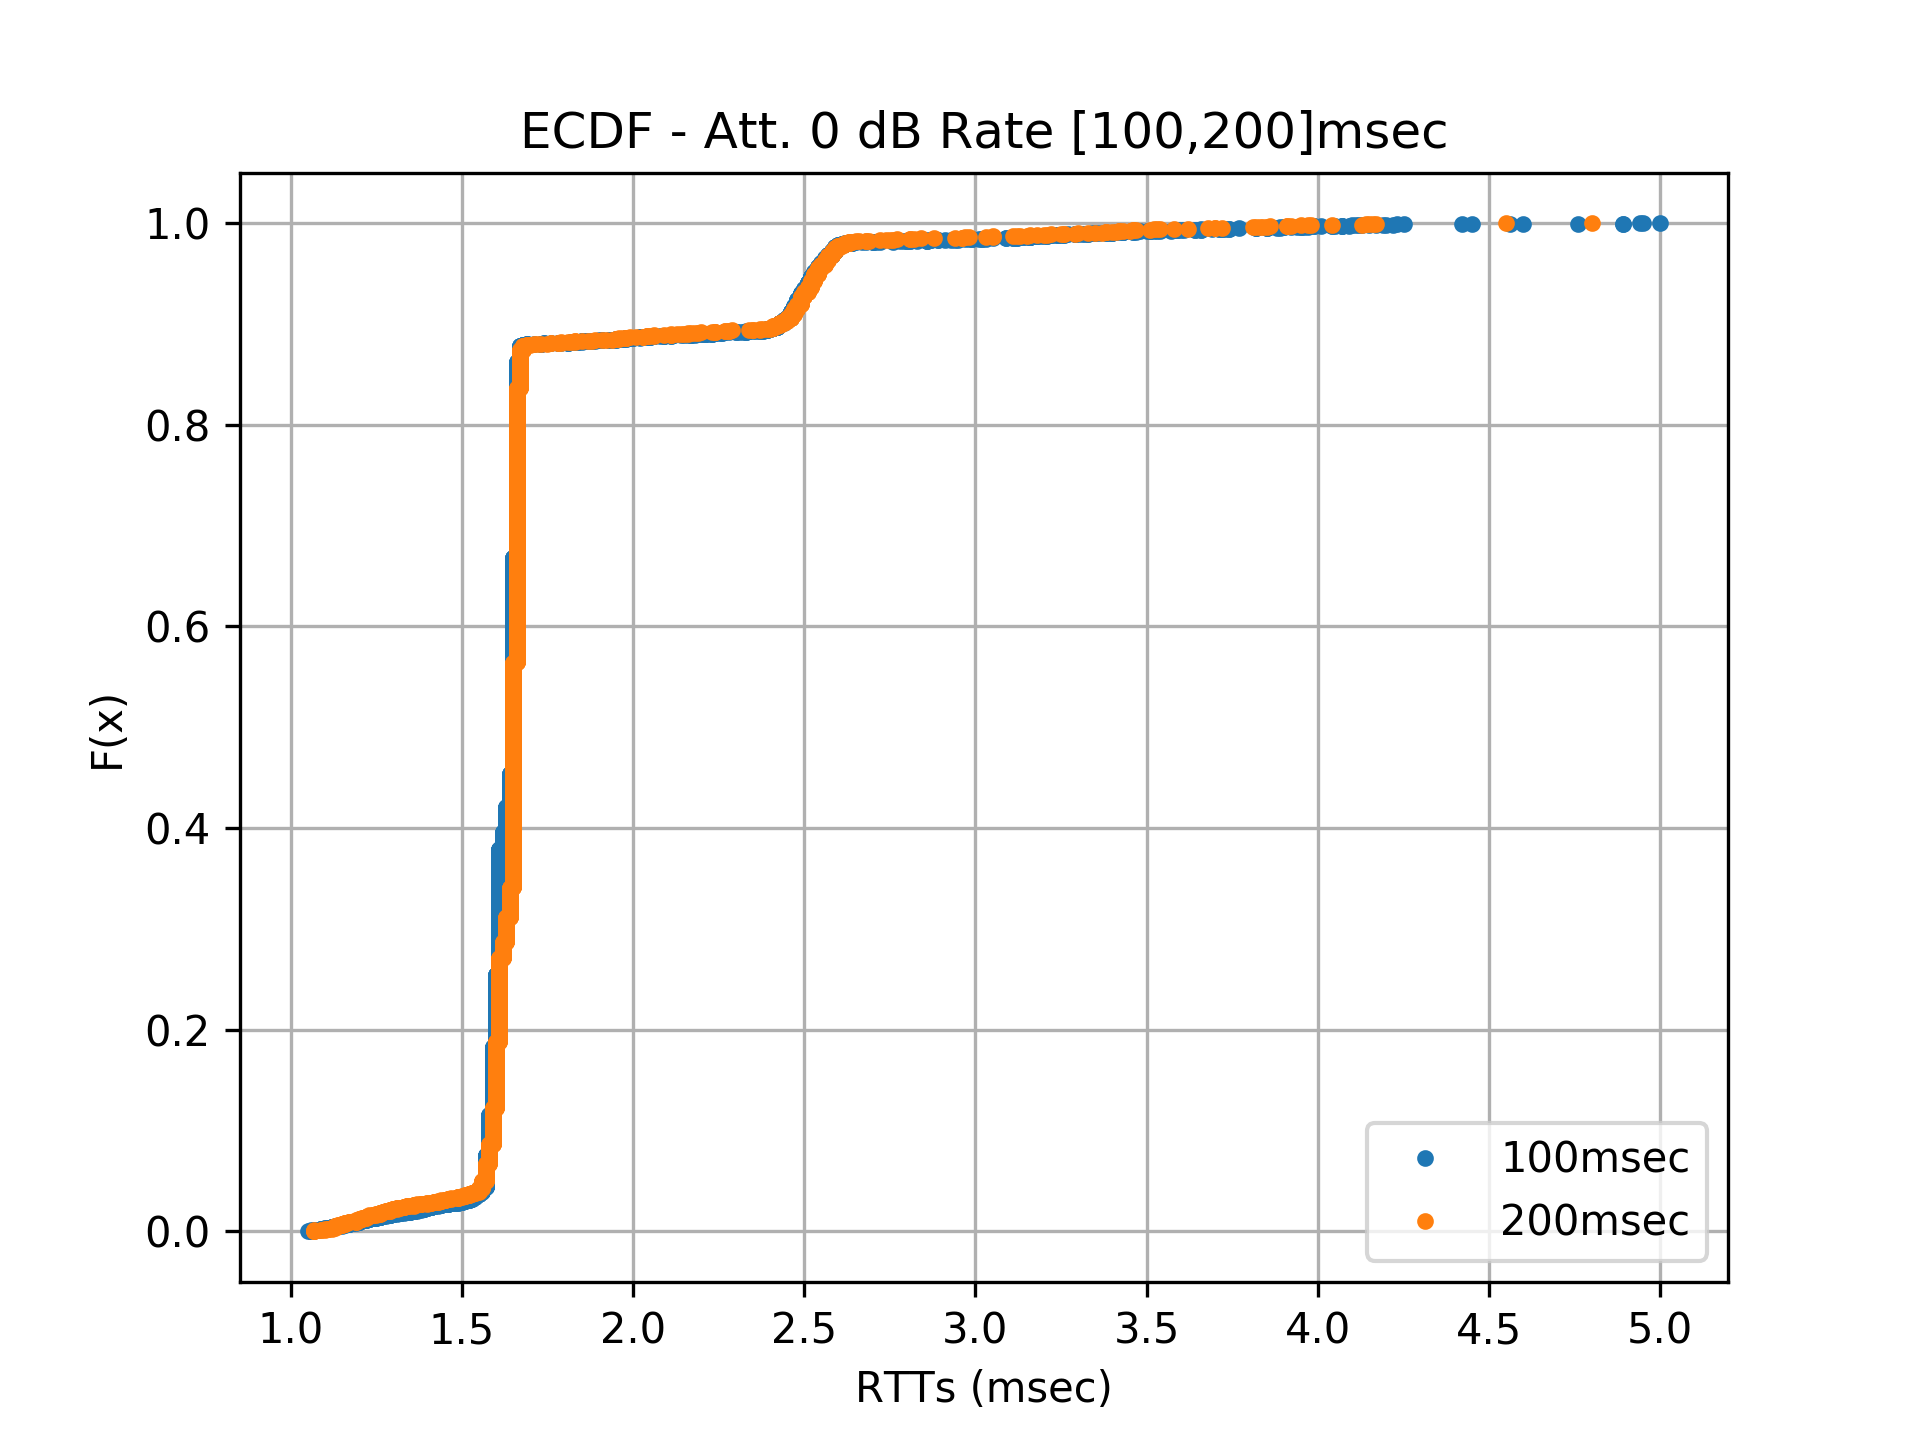
\includegraphics[width=8cm]{Rates_Atts/Att_0dBRate[100,200]msec}
	\caption{Att. 0 dBm - Rate 100,200 msec}
	\label{att_0_100and200msec}
\end{figure}

Figure \ref{rate_200msec_Att_0_15_30dBm} help us to validate an expected behavior. As we increase attenuation, the RTT is expected to be higher. This behavior is depicted in figure \ref{rate_200msec_Att_0_15_30dBm}.

\begin{figure}[h]
	\centering
	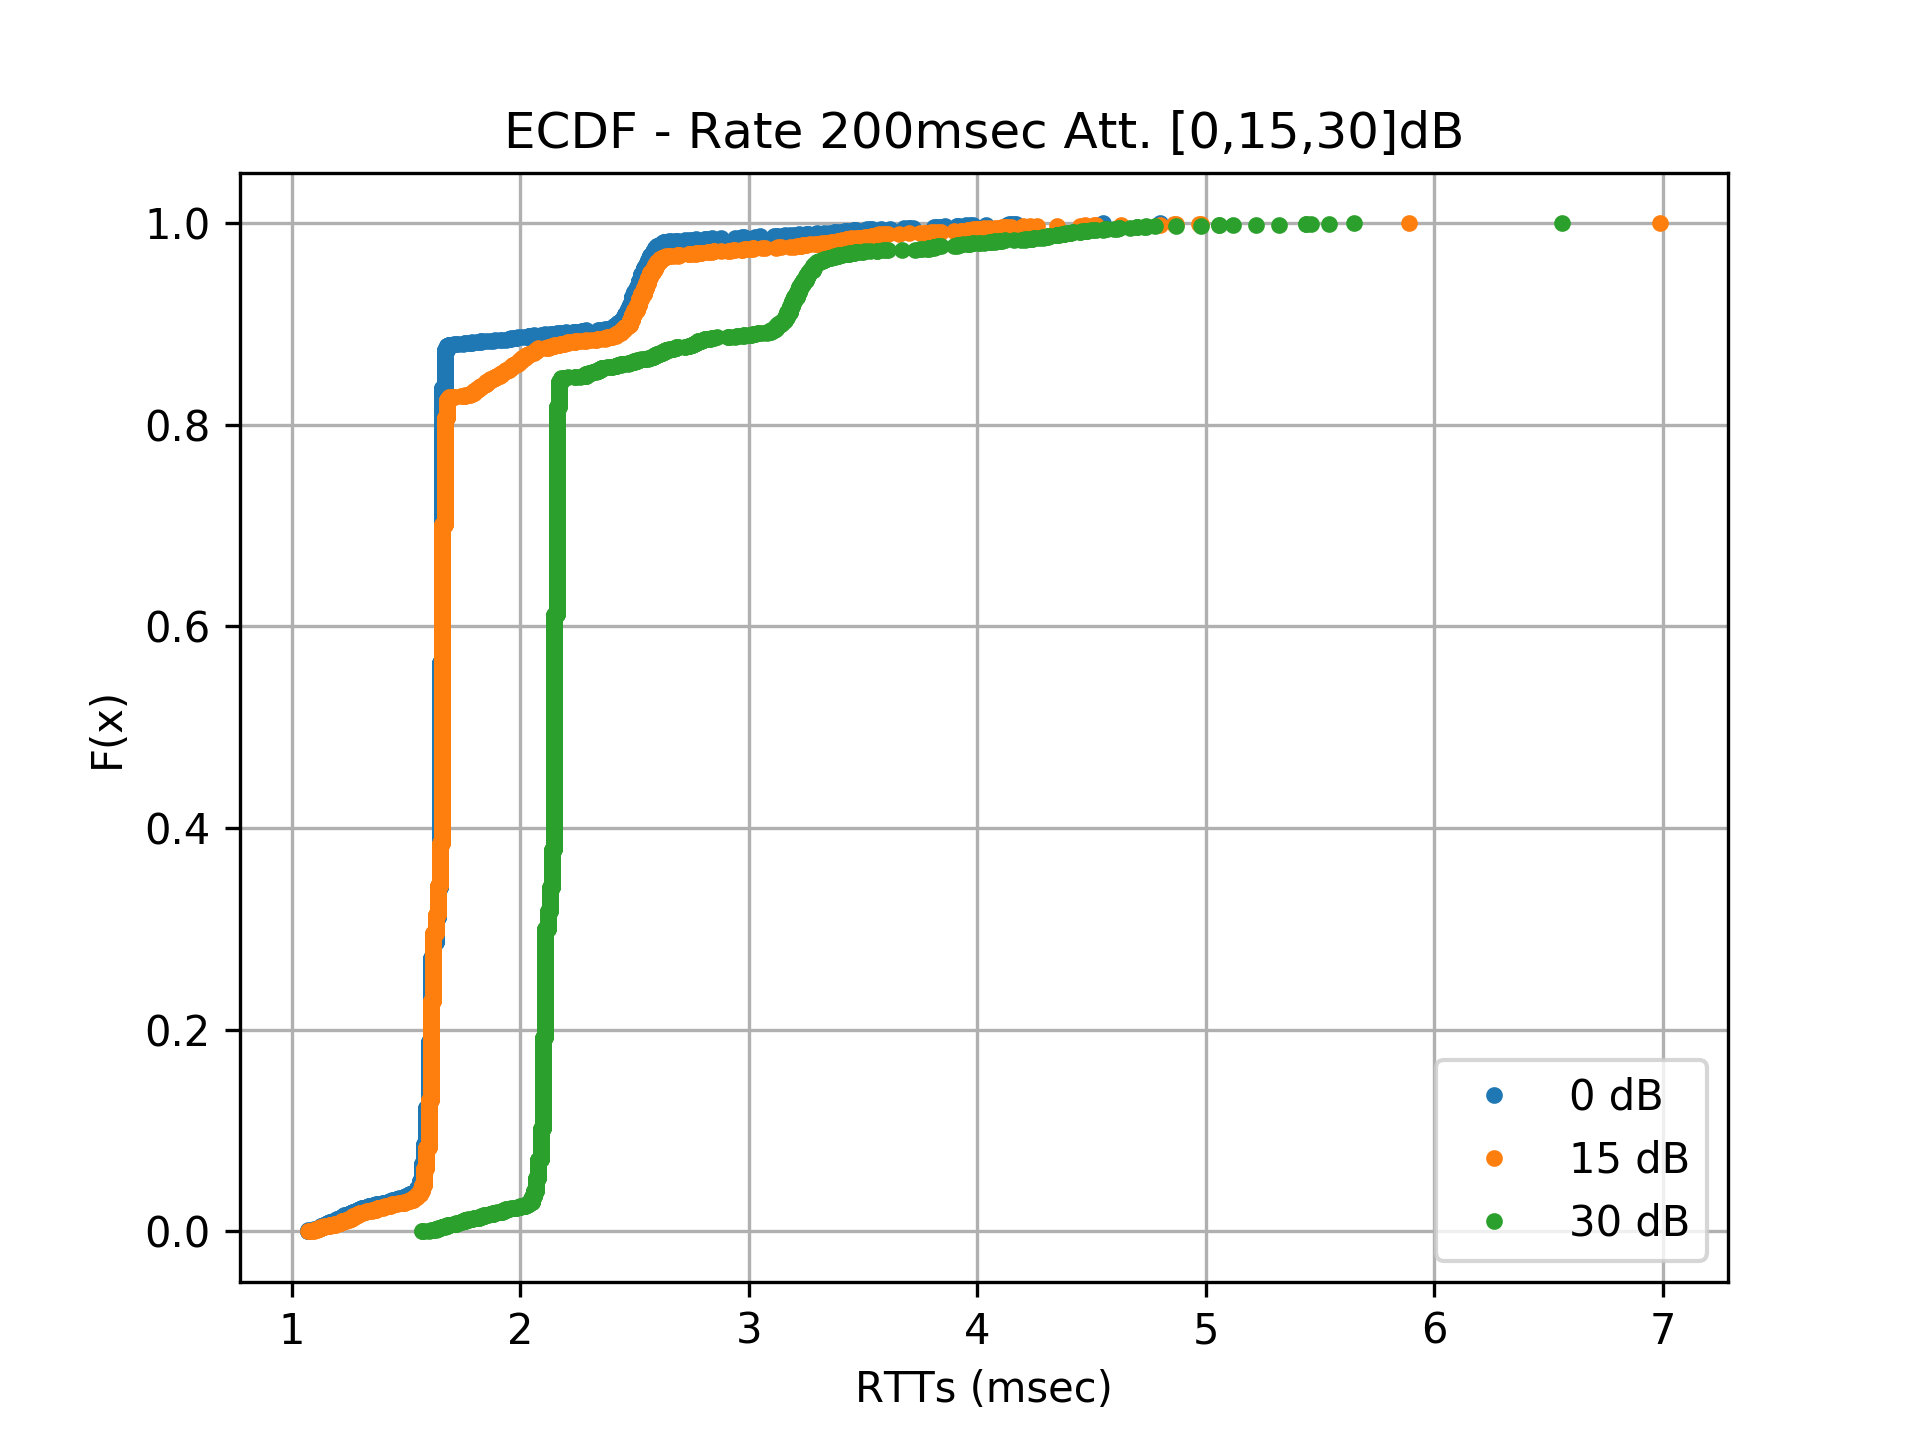
\includegraphics[width=8cm]{Rates_Atts/Rate200msecAtt_[0,15,30]dB}
	\caption{Rate 200 msec - Att. [0,15,30] dB}
	\label{rate_200msec_Att_0_15_30dBm}
\end{figure}

\emph{We can also describe that the p-value is close to 1 and the D-Value, which is the KS statistic is low. KS Low value is pursed as it means distance between the two ECDFs is small, meaning they are close to each other, hence more similar.}